\documentclass[12pt]{article}
\usepackage[margin=1in]{geometry} 
\usepackage{amsmath}
\usepackage{tcolorbox}
\usepackage{amssymb}
\usepackage{amsthm}
\usepackage{lastpage}
\usepackage{fancyhdr}
\usepackage{accents}
\pagestyle{fancy}
\setlength{\headheight}{40pt}


\newenvironment{solution}
  {\renewcommand\qedsymbol{$\blacksquare$}
  \begin{proof}[Solution]}
  {\end{proof}}
\renewcommand\qedsymbol{$\blacksquare$}

\newcommand{\ubar}[1]{\underaccent{\bar}{#1}}

\begin{document}

% Cover Page
\begin{titlepage}
  \centering
  
  {\scshape\LARGE University of British Columbia \par}
  \vspace{1cm}
  {\scshape\Large CPSC 425: Computer Vision\par}
  \vspace{1.5cm}
  {\huge\bfseries Assignment 3\par}
  \vspace{2cm}
  {\Large\itshape Simon Ghyselincks\par}
  \vfill
  Self-Studied based off of UBC CPSC 425 2023T1 course material\par

  \vfill

  % Bottom of the page
  {\large 2023\par}
\end{titlepage}

\lhead{UBC CPSC 425 Computer Vision: Assignment 3} 
\rhead{Term I 2023} 
\cfoot{\thepage\ of \pageref{LastPage}}

Based off of UBC CPSC 425 2023W T1 course material found at \texttt{https://mattabrown.github.io/425/assignments/Assignment3.html}

The goal is to implement an inpainting algorithm that finds patches with minimal SSD to fill in the missing pixels. The algorithm will be tested on the following image setup:

\begin{center}
  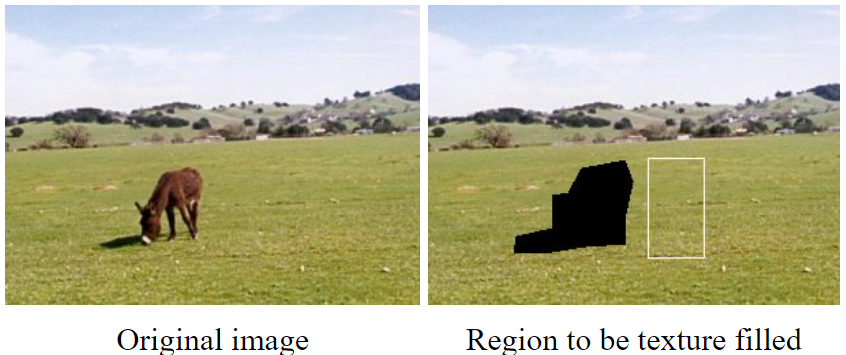
\includegraphics[width=0.65\textwidth]{imgs/1-premise.png}
\end{center}

The rest of the code for calculating SSD with a mask has been implemented to generate the following donkey removed image:

\begin{center}
  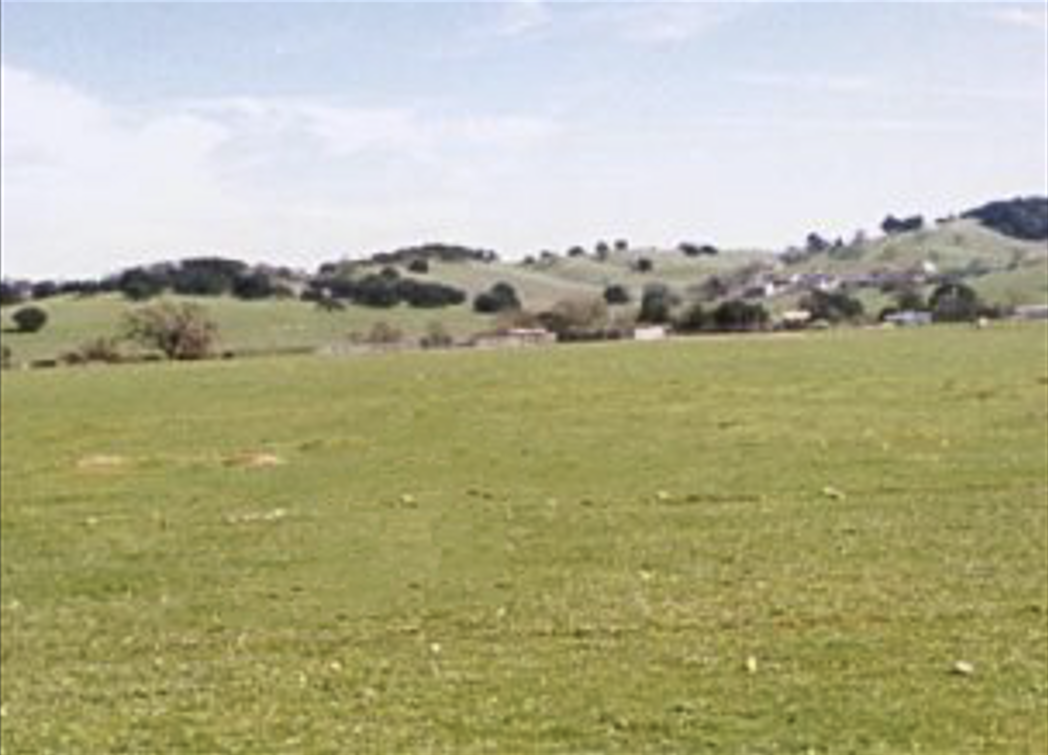
\includegraphics[width=0.65\textwidth]{imgs/5-donkeyfilled.png}
\end{center}

We can try and apply the same algorithm to a more challenging image:

\begin{center}
  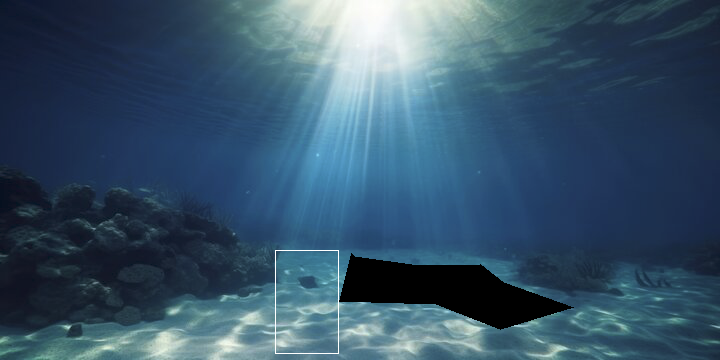
\includegraphics[width=0.65\textwidth]{imgs/6-ocean-clip.png}
\end{center}

The result is not as good as the donkey image, but a reasonable start. The smaller patch length of 2 helps to fill in the pixels better:
\begin{center}
  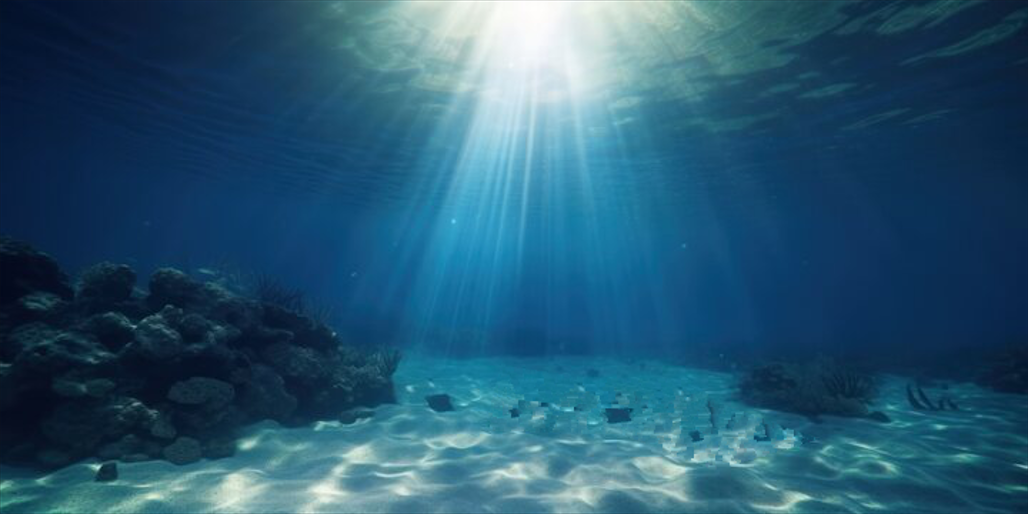
\includegraphics[width=0.65\textwidth]{imgs/6-ocean-fill.png}
\end{center}

Another experiment is to reduce the patch size even further so that it is only $3 \times 3$ pixels and also increase the std deviation of the potential patch randomization to $.8$ from $1$. This should create a smoother gradient between filled pixel patches. An issue with block patch sizes is that there are still biased vertical and horizontal lines that are visible. A single pixel at a time and a gaussian weighted window would improve this.

\begin{center}
  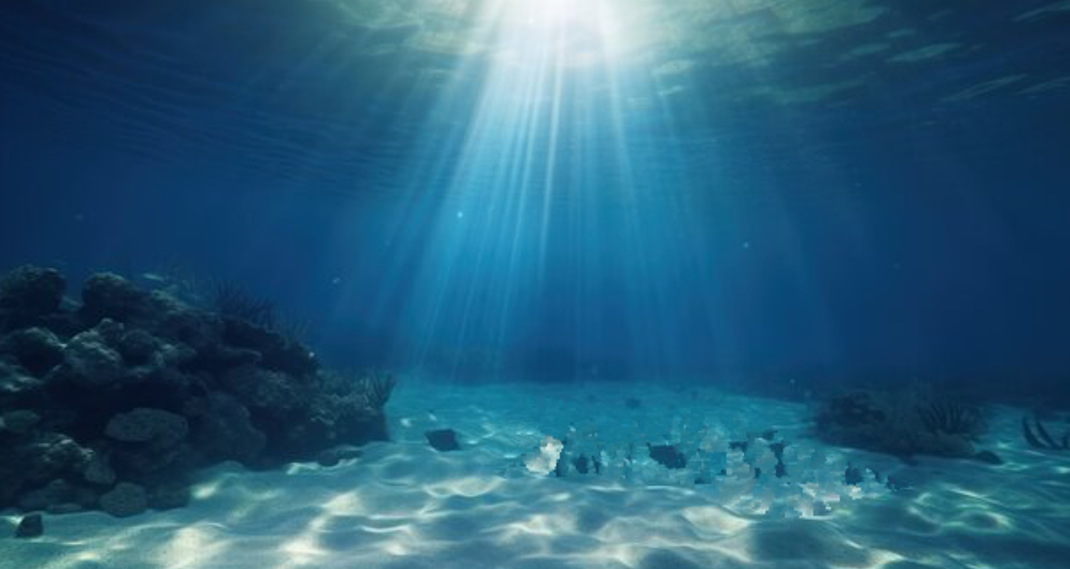
\includegraphics[width=0.65\textwidth]{imgs/6-ocean-fill-bad.png}
\end{center}

The result is rather dissapointing in the end with a more chaotic and noisy looking fill.
Overall, the piece with a stone is one of the few from the texture block that is at the right scale for the texturing so many pieces of the rock end up in the image.

\subsection*{Parameter Discussion:}

The randomPatchSD parameter applies to the standard deviation of the randomized selection of a patch from the minimum. We have a gaussian normal distribution when it comes to the probability of selecting an index from the ordered list of minimum SSD matches. A higher parameter value gives a higher chance of selecting the non-minimum patches and can add more variety to the texture. A lower value can give more consistency but also more repetition.

The patchL parameter is the length of a half-side of the patch. A smaller paramter can give too many edges that look like hard cuts since there is not as much natural variation in the texture and it is more mozaic-like at a finer scale. If the value is too large then the human eye can quickly percieve that entire sections of the image have been largely duplicated.

\end{document}